% Options for packages loaded elsewhere
\PassOptionsToPackage{unicode}{hyperref}
\PassOptionsToPackage{hyphens}{url}
%
\documentclass[
]{article}
\usepackage{lmodern}
\usepackage{amssymb,amsmath}
\usepackage{ifxetex,ifluatex}
\ifnum 0\ifxetex 1\fi\ifluatex 1\fi=0 % if pdftex
  \usepackage[T1]{fontenc}
  \usepackage[utf8]{inputenc}
  \usepackage{textcomp} % provide euro and other symbols
\else % if luatex or xetex
  \usepackage{unicode-math}
  \defaultfontfeatures{Scale=MatchLowercase}
  \defaultfontfeatures[\rmfamily]{Ligatures=TeX,Scale=1}
\fi
% Use upquote if available, for straight quotes in verbatim environments
\IfFileExists{upquote.sty}{\usepackage{upquote}}{}
\IfFileExists{microtype.sty}{% use microtype if available
  \usepackage[]{microtype}
  \UseMicrotypeSet[protrusion]{basicmath} % disable protrusion for tt fonts
}{}
\makeatletter
\@ifundefined{KOMAClassName}{% if non-KOMA class
  \IfFileExists{parskip.sty}{%
    \usepackage{parskip}
  }{% else
    \setlength{\parindent}{0pt}
    \setlength{\parskip}{6pt plus 2pt minus 1pt}}
}{% if KOMA class
  \KOMAoptions{parskip=half}}
\makeatother
\usepackage{xcolor}
\IfFileExists{xurl.sty}{\usepackage{xurl}}{} % add URL line breaks if available
\IfFileExists{bookmark.sty}{\usepackage{bookmark}}{\usepackage{hyperref}}
\hypersetup{
  pdftitle={Xbox game pass},
  pdfauthor={R.N.Madushika},
  hidelinks,
  pdfcreator={LaTeX via pandoc}}
\urlstyle{same} % disable monospaced font for URLs
\usepackage[margin=1in]{geometry}
\usepackage{color}
\usepackage{fancyvrb}
\newcommand{\VerbBar}{|}
\newcommand{\VERB}{\Verb[commandchars=\\\{\}]}
\DefineVerbatimEnvironment{Highlighting}{Verbatim}{commandchars=\\\{\}}
% Add ',fontsize=\small' for more characters per line
\usepackage{framed}
\definecolor{shadecolor}{RGB}{248,248,248}
\newenvironment{Shaded}{\begin{snugshade}}{\end{snugshade}}
\newcommand{\AlertTok}[1]{\textcolor[rgb]{0.94,0.16,0.16}{#1}}
\newcommand{\AnnotationTok}[1]{\textcolor[rgb]{0.56,0.35,0.01}{\textbf{\textit{#1}}}}
\newcommand{\AttributeTok}[1]{\textcolor[rgb]{0.77,0.63,0.00}{#1}}
\newcommand{\BaseNTok}[1]{\textcolor[rgb]{0.00,0.00,0.81}{#1}}
\newcommand{\BuiltInTok}[1]{#1}
\newcommand{\CharTok}[1]{\textcolor[rgb]{0.31,0.60,0.02}{#1}}
\newcommand{\CommentTok}[1]{\textcolor[rgb]{0.56,0.35,0.01}{\textit{#1}}}
\newcommand{\CommentVarTok}[1]{\textcolor[rgb]{0.56,0.35,0.01}{\textbf{\textit{#1}}}}
\newcommand{\ConstantTok}[1]{\textcolor[rgb]{0.00,0.00,0.00}{#1}}
\newcommand{\ControlFlowTok}[1]{\textcolor[rgb]{0.13,0.29,0.53}{\textbf{#1}}}
\newcommand{\DataTypeTok}[1]{\textcolor[rgb]{0.13,0.29,0.53}{#1}}
\newcommand{\DecValTok}[1]{\textcolor[rgb]{0.00,0.00,0.81}{#1}}
\newcommand{\DocumentationTok}[1]{\textcolor[rgb]{0.56,0.35,0.01}{\textbf{\textit{#1}}}}
\newcommand{\ErrorTok}[1]{\textcolor[rgb]{0.64,0.00,0.00}{\textbf{#1}}}
\newcommand{\ExtensionTok}[1]{#1}
\newcommand{\FloatTok}[1]{\textcolor[rgb]{0.00,0.00,0.81}{#1}}
\newcommand{\FunctionTok}[1]{\textcolor[rgb]{0.00,0.00,0.00}{#1}}
\newcommand{\ImportTok}[1]{#1}
\newcommand{\InformationTok}[1]{\textcolor[rgb]{0.56,0.35,0.01}{\textbf{\textit{#1}}}}
\newcommand{\KeywordTok}[1]{\textcolor[rgb]{0.13,0.29,0.53}{\textbf{#1}}}
\newcommand{\NormalTok}[1]{#1}
\newcommand{\OperatorTok}[1]{\textcolor[rgb]{0.81,0.36,0.00}{\textbf{#1}}}
\newcommand{\OtherTok}[1]{\textcolor[rgb]{0.56,0.35,0.01}{#1}}
\newcommand{\PreprocessorTok}[1]{\textcolor[rgb]{0.56,0.35,0.01}{\textit{#1}}}
\newcommand{\RegionMarkerTok}[1]{#1}
\newcommand{\SpecialCharTok}[1]{\textcolor[rgb]{0.00,0.00,0.00}{#1}}
\newcommand{\SpecialStringTok}[1]{\textcolor[rgb]{0.31,0.60,0.02}{#1}}
\newcommand{\StringTok}[1]{\textcolor[rgb]{0.31,0.60,0.02}{#1}}
\newcommand{\VariableTok}[1]{\textcolor[rgb]{0.00,0.00,0.00}{#1}}
\newcommand{\VerbatimStringTok}[1]{\textcolor[rgb]{0.31,0.60,0.02}{#1}}
\newcommand{\WarningTok}[1]{\textcolor[rgb]{0.56,0.35,0.01}{\textbf{\textit{#1}}}}
\usepackage{graphicx,grffile}
\makeatletter
\def\maxwidth{\ifdim\Gin@nat@width>\linewidth\linewidth\else\Gin@nat@width\fi}
\def\maxheight{\ifdim\Gin@nat@height>\textheight\textheight\else\Gin@nat@height\fi}
\makeatother
% Scale images if necessary, so that they will not overflow the page
% margins by default, and it is still possible to overwrite the defaults
% using explicit options in \includegraphics[width, height, ...]{}
\setkeys{Gin}{width=\maxwidth,height=\maxheight,keepaspectratio}
% Set default figure placement to htbp
\makeatletter
\def\fps@figure{htbp}
\makeatother
\setlength{\emergencystretch}{3em} % prevent overfull lines
\providecommand{\tightlist}{%
  \setlength{\itemsep}{0pt}\setlength{\parskip}{0pt}}
\setcounter{secnumdepth}{-\maxdimen} % remove section numbering
\usepackage{booktabs}
\usepackage{longtable}
\usepackage{array}
\usepackage{multirow}
\usepackage{wrapfig}
\usepackage{float}
\usepackage{colortbl}
\usepackage{pdflscape}
\usepackage{tabu}
\usepackage{threeparttable}
\usepackage{threeparttablex}
\usepackage[normalem]{ulem}
\usepackage{makecell}
\usepackage{xcolor}

\title{Xbox game pass}
\author{R.N.Madushika}
\date{5/8/2022}

\begin{document}
\maketitle

\begin{Shaded}
\begin{Highlighting}[]
\KeywordTok{set.seed}\NormalTok{(}\DecValTok{1233453}\NormalTok{)}
\end{Highlighting}
\end{Shaded}

\begin{Shaded}
\begin{Highlighting}[]
\KeywordTok{library}\NormalTok{(tidyverse)}
\end{Highlighting}
\end{Shaded}

\begin{verbatim}
## Warning: package 'tidyverse' was built under R version 4.0.5
\end{verbatim}

\begin{verbatim}
## -- Attaching packages --------------------------------------- tidyverse 1.3.1 --
\end{verbatim}

\begin{verbatim}
## v ggplot2 3.3.5     v purrr   0.3.4
## v tibble  3.1.6     v dplyr   1.0.7
## v tidyr   1.1.3     v stringr 1.4.0
## v readr   1.4.0     v forcats 0.5.1
\end{verbatim}

\begin{verbatim}
## Warning: package 'ggplot2' was built under R version 4.0.5
\end{verbatim}

\begin{verbatim}
## Warning: package 'tibble' was built under R version 4.0.5
\end{verbatim}

\begin{verbatim}
## Warning: package 'tidyr' was built under R version 4.0.5
\end{verbatim}

\begin{verbatim}
## Warning: package 'purrr' was built under R version 4.0.5
\end{verbatim}

\begin{verbatim}
## Warning: package 'dplyr' was built under R version 4.0.5
\end{verbatim}

\begin{verbatim}
## Warning: package 'forcats' was built under R version 4.0.5
\end{verbatim}

\begin{verbatim}
## -- Conflicts ------------------------------------------ tidyverse_conflicts() --
## x dplyr::filter() masks stats::filter()
## x dplyr::lag()    masks stats::lag()
\end{verbatim}

\begin{Shaded}
\begin{Highlighting}[]
\KeywordTok{library}\NormalTok{(BAS)}
\end{Highlighting}
\end{Shaded}

\begin{verbatim}
## Warning: package 'BAS' was built under R version 4.0.5
\end{verbatim}

\begin{Shaded}
\begin{Highlighting}[]
\KeywordTok{library}\NormalTok{(mice)}
\end{Highlighting}
\end{Shaded}

\begin{verbatim}
## Warning: package 'mice' was built under R version 4.0.5
\end{verbatim}

\begin{verbatim}
## 
## Attaching package: 'mice'
\end{verbatim}

\begin{verbatim}
## The following object is masked from 'package:stats':
## 
##     filter
\end{verbatim}

\begin{verbatim}
## The following objects are masked from 'package:base':
## 
##     cbind, rbind
\end{verbatim}

\begin{Shaded}
\begin{Highlighting}[]
\KeywordTok{library}\NormalTok{(dlookr)}
\end{Highlighting}
\end{Shaded}

\begin{verbatim}
## Warning: package 'dlookr' was built under R version 4.0.5
\end{verbatim}

\begin{verbatim}
## 
## Attaching package: 'dlookr'
\end{verbatim}

\begin{verbatim}
## The following object is masked from 'package:tidyr':
## 
##     extract
\end{verbatim}

\begin{verbatim}
## The following object is masked from 'package:base':
## 
##     transform
\end{verbatim}

\begin{Shaded}
\begin{Highlighting}[]
\KeywordTok{library}\NormalTok{(GGally)}
\end{Highlighting}
\end{Shaded}

\begin{verbatim}
## Warning: package 'GGally' was built under R version 4.0.5
\end{verbatim}

\begin{verbatim}
## Registered S3 method overwritten by 'GGally':
##   method from   
##   +.gg   ggplot2
\end{verbatim}

\begin{Shaded}
\begin{Highlighting}[]
\KeywordTok{library}\NormalTok{(caret)}
\end{Highlighting}
\end{Shaded}

\begin{verbatim}
## Warning: package 'caret' was built under R version 4.0.5
\end{verbatim}

\begin{verbatim}
## Loading required package: lattice
\end{verbatim}

\begin{verbatim}
## 
## Attaching package: 'caret'
\end{verbatim}

\begin{verbatim}
## The following object is masked from 'package:purrr':
## 
##     lift
\end{verbatim}

\begin{Shaded}
\begin{Highlighting}[]
\KeywordTok{library}\NormalTok{(readr)}
\NormalTok{Games <-}\StringTok{ }\KeywordTok{read_csv}\NormalTok{(}\StringTok{"C:/Users/Mani/Desktop/ST406/archive (7)/Gamepass_Games_v1.csv"}\NormalTok{)}
\end{Highlighting}
\end{Shaded}

\begin{verbatim}
## 
## -- Column specification --------------------------------------------------------
## cols(
##   GAME = col_character(),
##   RATIO = col_character(),
##   GAMERS = col_number(),
##   `COMP %` = col_double(),
##   TIME = col_character(),
##   RATING = col_double(),
##   ADDED = col_character(),
##   True_Achievement = col_double(),
##   Game_Score = col_double()
## )
\end{verbatim}

\begin{Shaded}
\begin{Highlighting}[]
\KeywordTok{View}\NormalTok{(Games)}
\NormalTok{Games <-}\StringTok{ }\KeywordTok{data.frame}\NormalTok{(Games)}
\end{Highlighting}
\end{Shaded}

\begin{Shaded}
\begin{Highlighting}[]
\CommentTok{#Structure of the dataset}
\KeywordTok{str}\NormalTok{(Games)}
\end{Highlighting}
\end{Shaded}

\begin{verbatim}
## 'data.frame':    455 obs. of  9 variables:
##  $ GAME            : chr  "Mass Effect Legendary Edition" "The Elder Scrolls V: Skyrim Special Edition" "Mass Effect 2" "Stardew Valley" ...
##  $ RATIO           : chr  "1.87" "1.97" "1.34" "3.04" ...
##  $ GAMERS          : num  84143 213257 221178 51530 71981 ...
##  $ COMP..          : num  4.1 8 9.6 1 15.6 6.1 9.8 3.8 0.9 1.9 ...
##  $ TIME            : chr  "100-120 hours" "80-100 hours" "50-60 hours" "150-200 hours" ...
##  $ RATING          : num  4.8 4.7 4.7 4.7 4.7 4.6 4.6 4.6 4.6 4.6 ...
##  $ ADDED           : chr  "06 Jan 22" "15 Dec 20" "09 Nov 20" "02 Dec 21" ...
##  $ True_Achievement: num  5442 3055 1819 3036 1678 ...
##  $ Game_Score      : num  2915 1550 1355 1000 1000 ...
\end{verbatim}

\begin{Shaded}
\begin{Highlighting}[]
\KeywordTok{head}\NormalTok{(Games)}
\end{Highlighting}
\end{Shaded}

\begin{verbatim}
##                                          GAME RATIO GAMERS COMP..          TIME
## 1               Mass Effect Legendary Edition  1.87  84143    4.1 100-120 hours
## 2 The Elder Scrolls V: Skyrim Special Edition  1.97 213257    8.0  80-100 hours
## 3                               Mass Effect 2  1.34 221178    9.6   50-60 hours
## 4                              Stardew Valley  3.04  51530    1.0 150-200 hours
## 5                                It Takes Two  1.68  71981   15.6   12-15 hours
## 6                                       Hades  2.40  83710    6.1   60-80 hours
##   RATING     ADDED True_Achievement Game_Score
## 1    4.8 06 Jan 22             5442       2915
## 2    4.7 15 Dec 20             3055       1550
## 3    4.7 09 Nov 20             1819       1355
## 4    4.7 02 Dec 21             3036       1000
## 5    4.7 03 Nov 21             1678       1000
## 6    4.6 18 Jun 21             2404       1000
\end{verbatim}

\begin{Shaded}
\begin{Highlighting}[]
\KeywordTok{summary}\NormalTok{(Games)}
\end{Highlighting}
\end{Shaded}

\begin{verbatim}
##      GAME              RATIO               GAMERS           COMP..      
##  Length:455         Length:455         Min.   :     0   Min.   : 0.000  
##  Class :character   Class :character   1st Qu.: 17781   1st Qu.: 0.600  
##  Mode  :character   Mode  :character   Median : 52268   Median : 1.900  
##                                        Mean   : 83540   Mean   : 6.345  
##                                        3rd Qu.:116796   3rd Qu.: 6.100  
##                                        Max.   :455839   Max.   :84.700  
##                                                                         
##      TIME               RATING         ADDED           True_Achievement
##  Length:455         Min.   :2.000   Length:455         Min.   :  252   
##  Class :character   1st Qu.:3.400   Class :character   1st Qu.: 2102   
##  Mode  :character   Median :3.700   Mode  :character   Median : 3231   
##                     Mean   :3.702                      Mean   : 4693   
##                     3rd Qu.:4.100                      3rd Qu.: 4995   
##                     Max.   :4.800                      Max.   :37178   
##                     NA's   :3                                          
##    Game_Score  
##  Min.   : 200  
##  1st Qu.:1000  
##  Median :1000  
##  Mean   :1209  
##  3rd Qu.:1212  
##  Max.   :7000  
## 
\end{verbatim}

\begin{Shaded}
\begin{Highlighting}[]
\CommentTok{#data cleaning}

\CommentTok{#Remove duplicates}
\NormalTok{Games <-}\StringTok{ }\NormalTok{Games[}\OperatorTok{!}\KeywordTok{duplicated}\NormalTok{(Games}\OperatorTok{$}\NormalTok{GAME), ]}

\CommentTok{#Check for missing values}
\KeywordTok{sum}\NormalTok{(}\KeywordTok{is.na}\NormalTok{(Games))}
\end{Highlighting}
\end{Shaded}

\begin{verbatim}
## [1] 38
\end{verbatim}

\begin{Shaded}
\begin{Highlighting}[]
\CommentTok{#remove the column with high missing values}
\NormalTok{Games =}\StringTok{ }\KeywordTok{subset}\NormalTok{(Games, }\DataTypeTok{select =} \OperatorTok{-}\KeywordTok{c}\NormalTok{(TIME) )}
\CommentTok{#Games}
\end{Highlighting}
\end{Shaded}

\begin{Shaded}
\begin{Highlighting}[]
\CommentTok{#remove rows with missing values}
\NormalTok{Games <-}\StringTok{ }\NormalTok{Games }\OperatorTok\StringTok{ }\KeywordTok{drop_na}\NormalTok{()}
\CommentTok{#Games}
\end{Highlighting}
\end{Shaded}

\begin{Shaded}
\begin{Highlighting}[]
\NormalTok{Games}\OperatorTok{$}\NormalTok{RATIO <-}\StringTok{ }\KeywordTok{as.numeric}\NormalTok{(Games}\OperatorTok{$}\NormalTok{RATIO)}
\CommentTok{#Games}
\end{Highlighting}
\end{Shaded}

\begin{Shaded}
\begin{Highlighting}[]
\CommentTok{#Exploratory data analysis}
\KeywordTok{describe}\NormalTok{(Games)}
\end{Highlighting}
\end{Shaded}

\begin{verbatim}
## # A tibble: 6 x 26
##   described_variables     n    na   mean      sd se_mean     IQR skewness kurtosis
##   <chr>               <int> <int>  <dbl>   <dbl>   <dbl>   <dbl>    <dbl>    <dbl>
## 1 RATIO                 449     0 3.73e0 3.02e+0 1.43e-1 2.05e+0    4.67    37.9  
## 2 GAMERS                449     0 8.43e4 8.87e+4 4.19e+3 1.01e+5    1.62     2.44 
## 3 COMP..                449     0 6.42e0 1.16e+1 5.49e-1 5.7 e+0    3.44    14.2  
## 4 RATING                449     0 3.70e0 5.14e-1 2.43e-2 7.  e-1   -0.504    0.168
## 5 True_Achievement      449     0 4.68e3 4.96e+3 2.34e+2 2.84e+3    3.51    15.3  
## 6 Game_Score            449     0 1.21e3 6.64e+2 3.13e+1 2.15e+2    4.07    23.6  
## # ... with 17 more variables: p00 <dbl>, p01 <dbl>, p05 <dbl>, p10 <dbl>,
## #   p20 <dbl>, p25 <dbl>, p30 <dbl>, p40 <dbl>, p50 <dbl>, p60 <dbl>,
## #   p70 <dbl>, p75 <dbl>, p80 <dbl>, p90 <dbl>, p95 <dbl>, p99 <dbl>,
## #   p100 <dbl>
\end{verbatim}

\begin{Shaded}
\begin{Highlighting}[]
\CommentTok{#Scatter plots}
\KeywordTok{ggplot}\NormalTok{(Games, }\KeywordTok{aes}\NormalTok{(}\DataTypeTok{x=}\NormalTok{RATIO, }\DataTypeTok{y=}\NormalTok{RATING)) }\OperatorTok{+}\StringTok{ }\KeywordTok{geom_point}\NormalTok{(}\DataTypeTok{color=}\StringTok{"blue"}\NormalTok{)}
\end{Highlighting}
\end{Shaded}

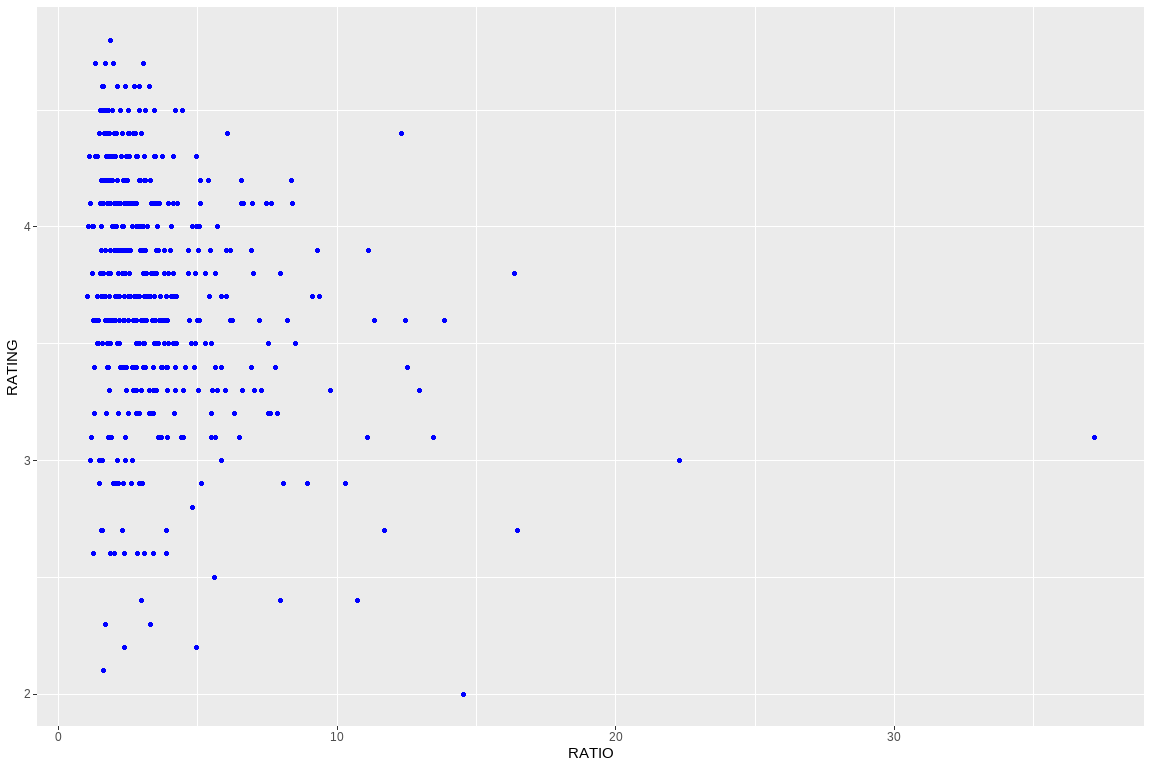
\includegraphics{Xbox_Games_Pass_files/figure-latex/unnamed-chunk-11-1.pdf}

\begin{Shaded}
\begin{Highlighting}[]
\KeywordTok{ggplot}\NormalTok{(Games, }\KeywordTok{aes}\NormalTok{(}\DataTypeTok{x=}\NormalTok{GAMERS, }\DataTypeTok{y=}\NormalTok{RATING)) }\OperatorTok{+}\StringTok{ }\KeywordTok{geom_point}\NormalTok{(}\DataTypeTok{color=}\StringTok{"blue"}\NormalTok{)}
\end{Highlighting}
\end{Shaded}

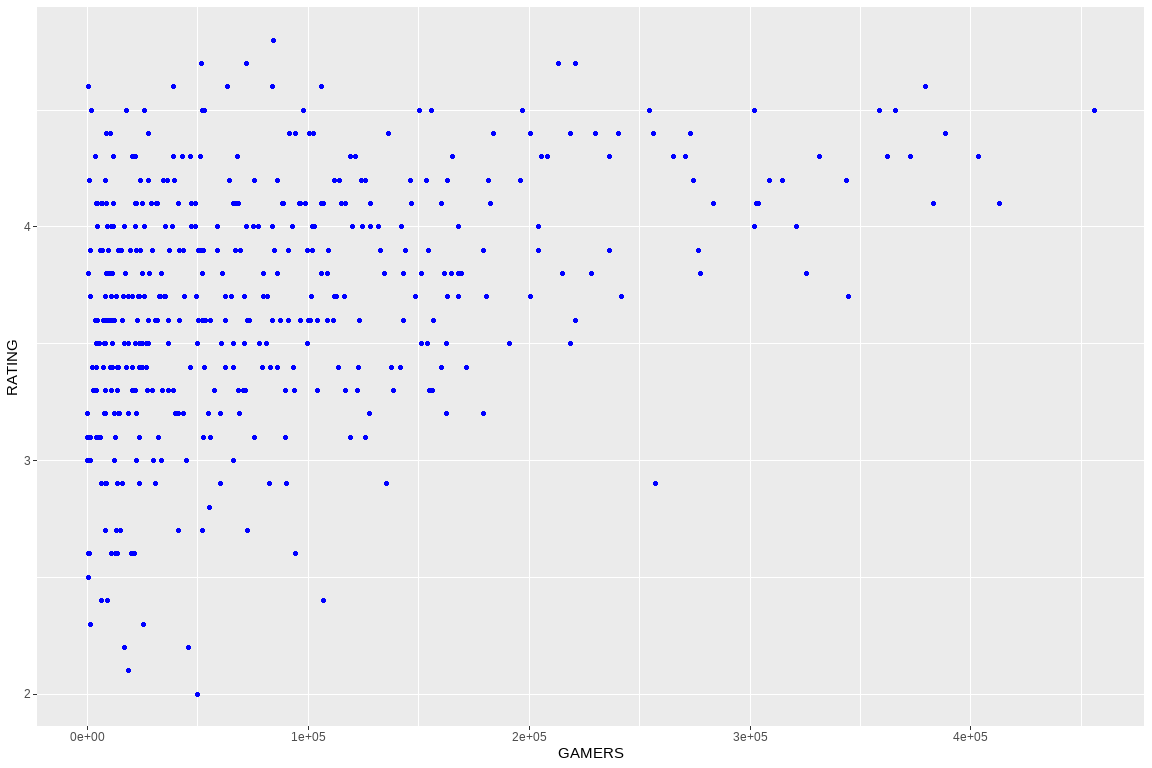
\includegraphics{Xbox_Games_Pass_files/figure-latex/unnamed-chunk-11-2.pdf}

\begin{Shaded}
\begin{Highlighting}[]
\KeywordTok{ggplot}\NormalTok{(Games, }\KeywordTok{aes}\NormalTok{(}\DataTypeTok{x=}\NormalTok{COMP.., }\DataTypeTok{y=}\NormalTok{RATING)) }\OperatorTok{+}\StringTok{ }\KeywordTok{geom_point}\NormalTok{(}\DataTypeTok{color=}\StringTok{"blue"}\NormalTok{)}
\end{Highlighting}
\end{Shaded}

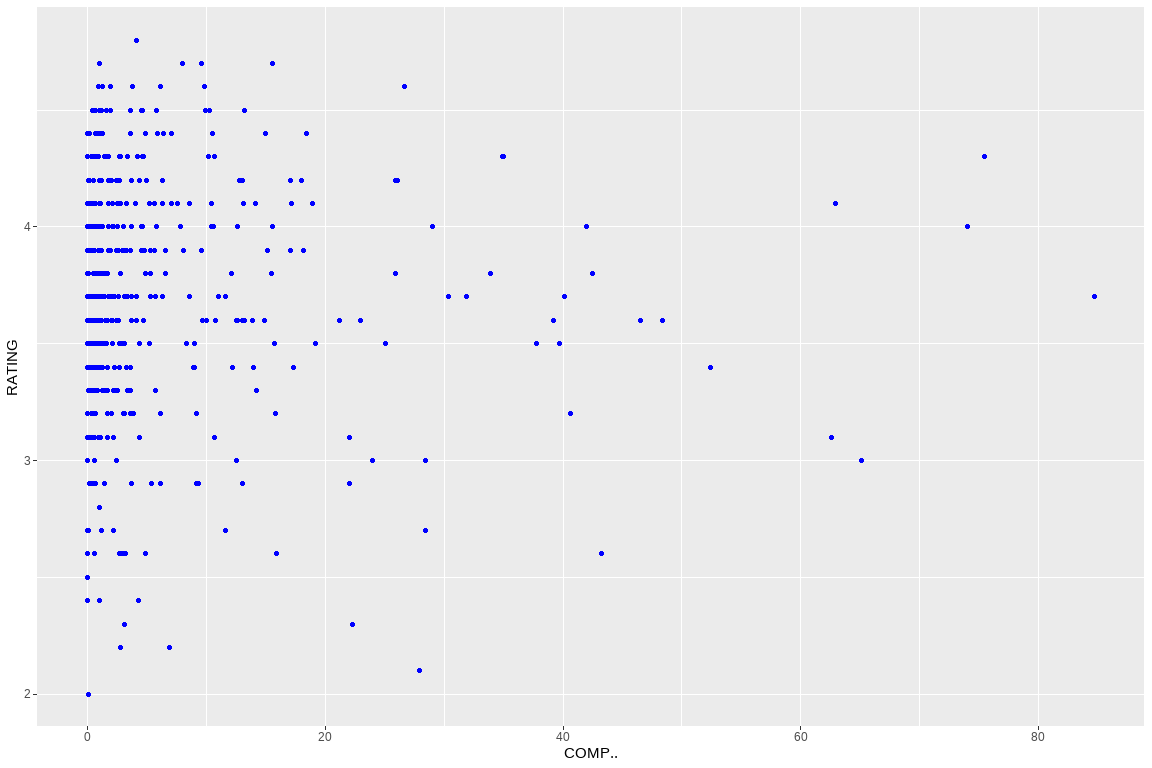
\includegraphics{Xbox_Games_Pass_files/figure-latex/unnamed-chunk-11-3.pdf}

\begin{Shaded}
\begin{Highlighting}[]
\KeywordTok{ggplot}\NormalTok{(Games, }\KeywordTok{aes}\NormalTok{(}\DataTypeTok{x=}\NormalTok{True_Achievement,}\DataTypeTok{y=}\NormalTok{RATING)) }\OperatorTok{+}\StringTok{ }\KeywordTok{geom_point}\NormalTok{(}\DataTypeTok{color=}\StringTok{"blue"}\NormalTok{)}
\end{Highlighting}
\end{Shaded}

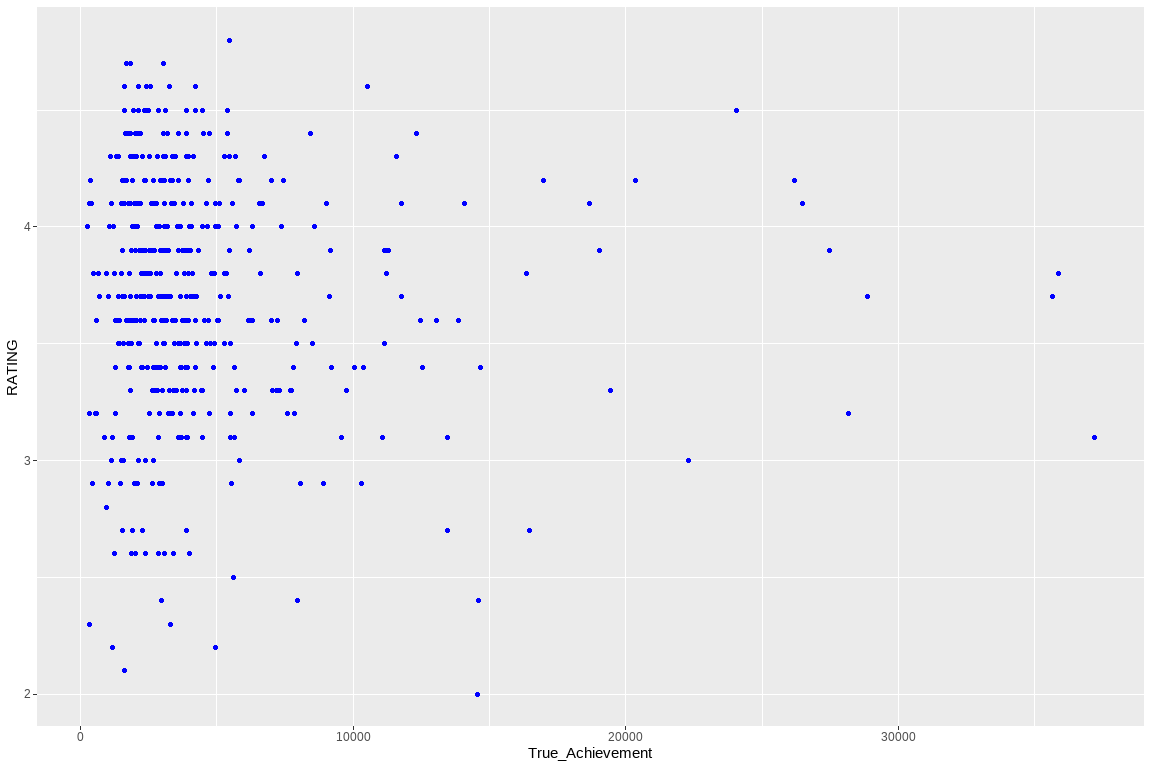
\includegraphics{Xbox_Games_Pass_files/figure-latex/unnamed-chunk-11-4.pdf}

\begin{Shaded}
\begin{Highlighting}[]
\KeywordTok{ggplot}\NormalTok{(Games, }\KeywordTok{aes}\NormalTok{(}\DataTypeTok{x=}\NormalTok{Game_Score, }\DataTypeTok{y=}\NormalTok{RATING)) }\OperatorTok{+}\StringTok{ }\KeywordTok{geom_point}\NormalTok{(}\DataTypeTok{color=}\StringTok{"blue"}\NormalTok{)}
\end{Highlighting}
\end{Shaded}

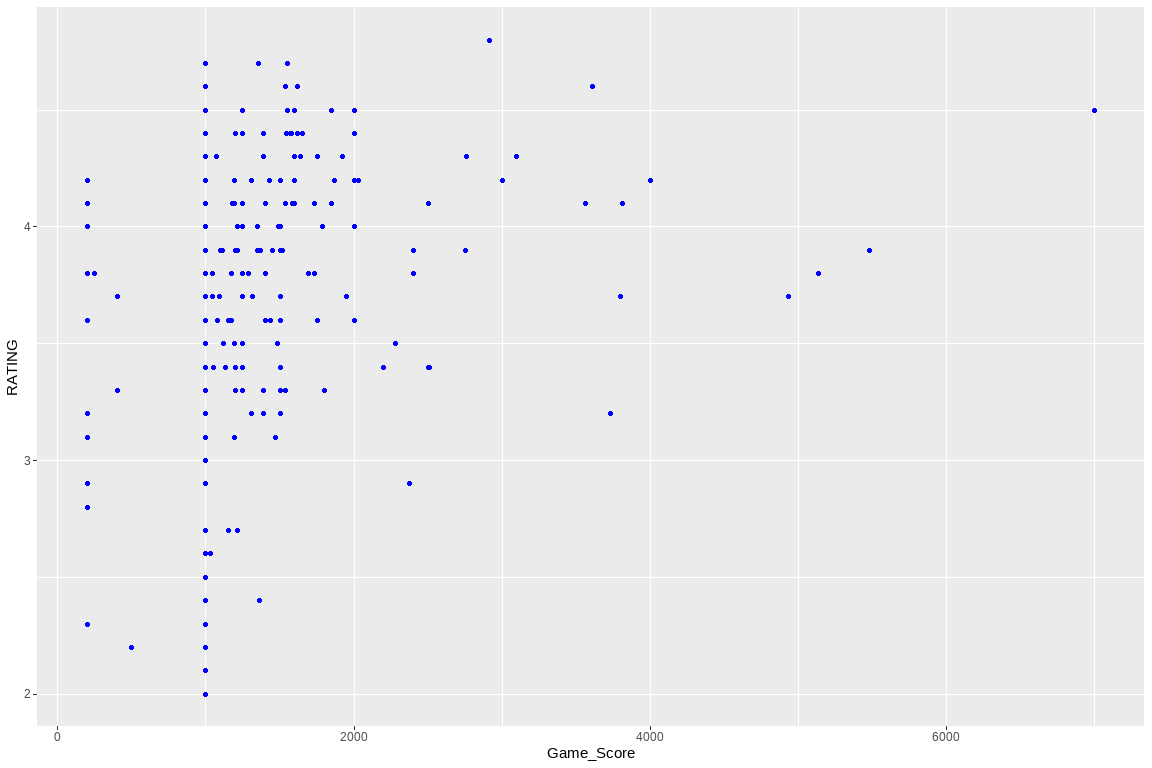
\includegraphics{Xbox_Games_Pass_files/figure-latex/unnamed-chunk-11-5.pdf}

\begin{Shaded}
\begin{Highlighting}[]
\CommentTok{#Find all correlations}
\KeywordTok{ggpairs}\NormalTok{(Games[}\OperatorTok{-}\KeywordTok{c}\NormalTok{(}\DecValTok{1}\NormalTok{,}\DecValTok{6}\NormalTok{)],)}
\end{Highlighting}
\end{Shaded}

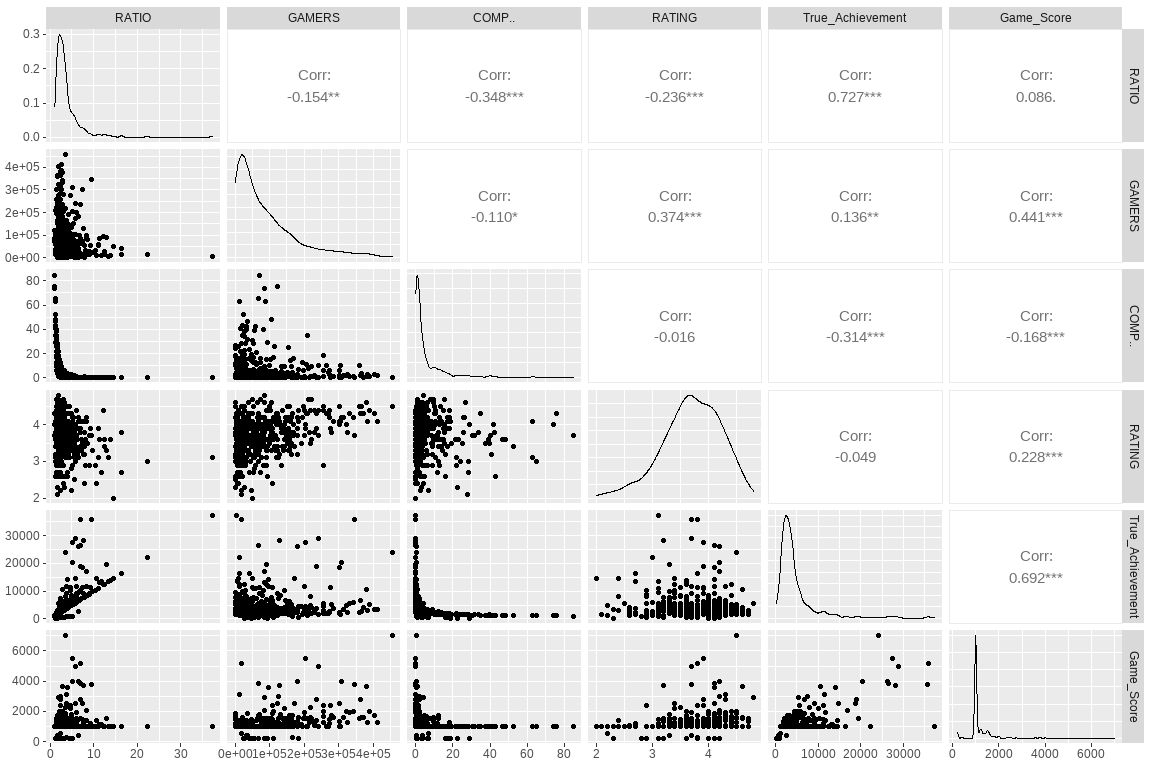
\includegraphics{Xbox_Games_Pass_files/figure-latex/unnamed-chunk-12-1.pdf}

\begin{Shaded}
\begin{Highlighting}[]
\CommentTok{#Building a model}
\CommentTok{#split data into training and test data sets}
\NormalTok{indxTrain <-}\StringTok{ }\KeywordTok{createDataPartition}\NormalTok{(}\DataTypeTok{y =}\NormalTok{ Games}\OperatorTok{$}\NormalTok{RATING,}\DataTypeTok{p =} \FloatTok{0.75}\NormalTok{,}\DataTypeTok{list =} \OtherTok{FALSE}\NormalTok{)}
\NormalTok{training <-}\StringTok{ }\NormalTok{Games[indxTrain,]}
\NormalTok{testing <-}\StringTok{ }\NormalTok{Games[}\OperatorTok{-}\NormalTok{indxTrain,]}
\CommentTok{#Check dimensions of the split}
\KeywordTok{prop.table}\NormalTok{(}\KeywordTok{table}\NormalTok{(Games}\OperatorTok{$}\NormalTok{RATING)) }\OperatorTok{*}\StringTok{ }\DecValTok{100}
\end{Highlighting}
\end{Shaded}

\begin{verbatim}
## 
##         2       2.1       2.2       2.3       2.4       2.5       2.6       2.7 
## 0.2227171 0.2227171 0.4454343 0.4454343 0.6681514 0.2227171 1.7817372 1.3363029 
##       2.8       2.9         3       3.1       3.2       3.3       3.4       3.5 
## 0.2227171 2.6726058 1.7817372 3.5634744 3.7861915 5.5679287 6.0133630 5.5679287 
##       3.6       3.7       3.8       3.9         4       4.1       4.2       4.3 
## 9.7995546 7.7951002 6.4587973 7.1269488 6.4587973 8.0178174 5.3452116 4.8997773 
##       4.4       4.5       4.6       4.7       4.8 
## 3.7861915 3.1180401 1.5590200 0.8908686 0.2227171
\end{verbatim}

\begin{Shaded}
\begin{Highlighting}[]
\KeywordTok{prop.table}\NormalTok{(}\KeywordTok{table}\NormalTok{(training}\OperatorTok{$}\NormalTok{RATING)) }\OperatorTok{*}\StringTok{ }\DecValTok{100}
\end{Highlighting}
\end{Shaded}

\begin{verbatim}
## 
##      2.1      2.2      2.3      2.4      2.6      2.7      2.8      2.9 
## 0.295858 0.591716 0.295858 0.591716 1.479290 1.183432 0.295858 2.366864 
##        3      3.1      3.2      3.3      3.4      3.5      3.6      3.7 
## 2.366864 4.142012 4.142012 5.325444 5.917160 6.213018 9.763314 7.100592 
##      3.8      3.9        4      4.1      4.2      4.3      4.4      4.5 
## 6.213018 7.988166 6.804734 7.100592 5.325444 4.733728 3.550296 2.958580 
##      4.6      4.7      4.8 
## 1.775148 1.183432 0.295858
\end{verbatim}

\begin{Shaded}
\begin{Highlighting}[]
\KeywordTok{prop.table}\NormalTok{(}\KeywordTok{table}\NormalTok{(testing}\OperatorTok{$}\NormalTok{RATING)) }\OperatorTok{*}\StringTok{ }\DecValTok{100}
\end{Highlighting}
\end{Shaded}

\begin{verbatim}
## 
##          2        2.3        2.4        2.5        2.6        2.7        2.9 
##  0.9009009  0.9009009  0.9009009  0.9009009  2.7027027  1.8018018  3.6036036 
##        3.1        3.2        3.3        3.4        3.5        3.6        3.7 
##  1.8018018  2.7027027  6.3063063  6.3063063  3.6036036  9.9099099  9.9099099 
##        3.8        3.9          4        4.1        4.2        4.3        4.4 
##  7.2072072  4.5045045  5.4054054 10.8108108  5.4054054  5.4054054  4.5045045 
##        4.5        4.6 
##  3.6036036  0.9009009
\end{verbatim}

\begin{Shaded}
\begin{Highlighting}[]
\CommentTok{#Bayesian Multiple Regression Model}

\NormalTok{Games.bas =}\StringTok{ }\KeywordTok{bas.lm}\NormalTok{(RATING }\OperatorTok{~}\StringTok{ }\NormalTok{., }\DataTypeTok{data =}\NormalTok{ training[}\OperatorTok{-}\KeywordTok{c}\NormalTok{(}\DecValTok{1}\NormalTok{,}\DecValTok{6}\NormalTok{)], }\DataTypeTok{prior =} \StringTok{"BIC"}\NormalTok{,}

\DataTypeTok{modelprior =}\KeywordTok{tr.beta.binomial}\NormalTok{(}\DecValTok{1}\NormalTok{,}\DecValTok{1}\NormalTok{,}\DecValTok{5}\NormalTok{),}
\DataTypeTok{include.always =} \OperatorTok{~}\StringTok{ }\NormalTok{.,}
\DataTypeTok{n.models =} \DecValTok{1}\NormalTok{)}

\NormalTok{Games.bas}
\end{Highlighting}
\end{Shaded}

\begin{verbatim}
## 
## Call:
## bas.lm(formula = RATING ~ ., data = training[-c(1, 6)], n.models = 1, 
##     prior = "BIC", modelprior = tr.beta.binomial(1, 1, 5), include.always = ~.)
## 
## 
##  Marginal Posterior Inclusion Probabilities: 
##        Intercept             RATIO            GAMERS            COMP..  
##                1                 1                 1                 1  
## True_Achievement        Game_Score  
##                1                 1
\end{verbatim}

\begin{Shaded}
\begin{Highlighting}[]
\NormalTok{Games.coef =}\StringTok{ }\KeywordTok{coef}\NormalTok{(Games.bas)}
\NormalTok{Games.coef}
\end{Highlighting}
\end{Shaded}

\begin{verbatim}
## 
##  Marginal Posterior Summaries of Coefficients: 
## 
##  Using  BMA 
## 
##  Based on the top  1 models 
##                   post mean   post SD     post p(B != 0)
## Intercept          3.707e+00   2.528e-02   1.000e+00    
## RATIO              1.232e-04   2.276e-02   1.000e+00    
## GAMERS             1.460e-06   3.392e-07   1.000e+00    
## COMP..            -2.808e-03   2.477e-03   1.000e+00    
## True_Achievement  -3.064e-05   1.914e-05   1.000e+00    
## Game_Score         2.255e-04   9.987e-05   1.000e+00
\end{verbatim}

\begin{Shaded}
\begin{Highlighting}[]
\KeywordTok{par}\NormalTok{(}\DataTypeTok{mfrow =} \KeywordTok{c}\NormalTok{(}\DecValTok{3}\NormalTok{, }\DecValTok{3}\NormalTok{), }\DataTypeTok{col.lab =} \StringTok{"darkgrey"}\NormalTok{, }\DataTypeTok{col.axis =} \StringTok{"darkgrey"}\NormalTok{, }\DataTypeTok{col =} \StringTok{"darkgrey"}\NormalTok{)}
\KeywordTok{plot}\NormalTok{(Games.coef, }\DataTypeTok{subset =} \DecValTok{2}\OperatorTok{:}\DecValTok{6}\NormalTok{, }\DataTypeTok{ask =}\NormalTok{ F)}
\end{Highlighting}
\end{Shaded}

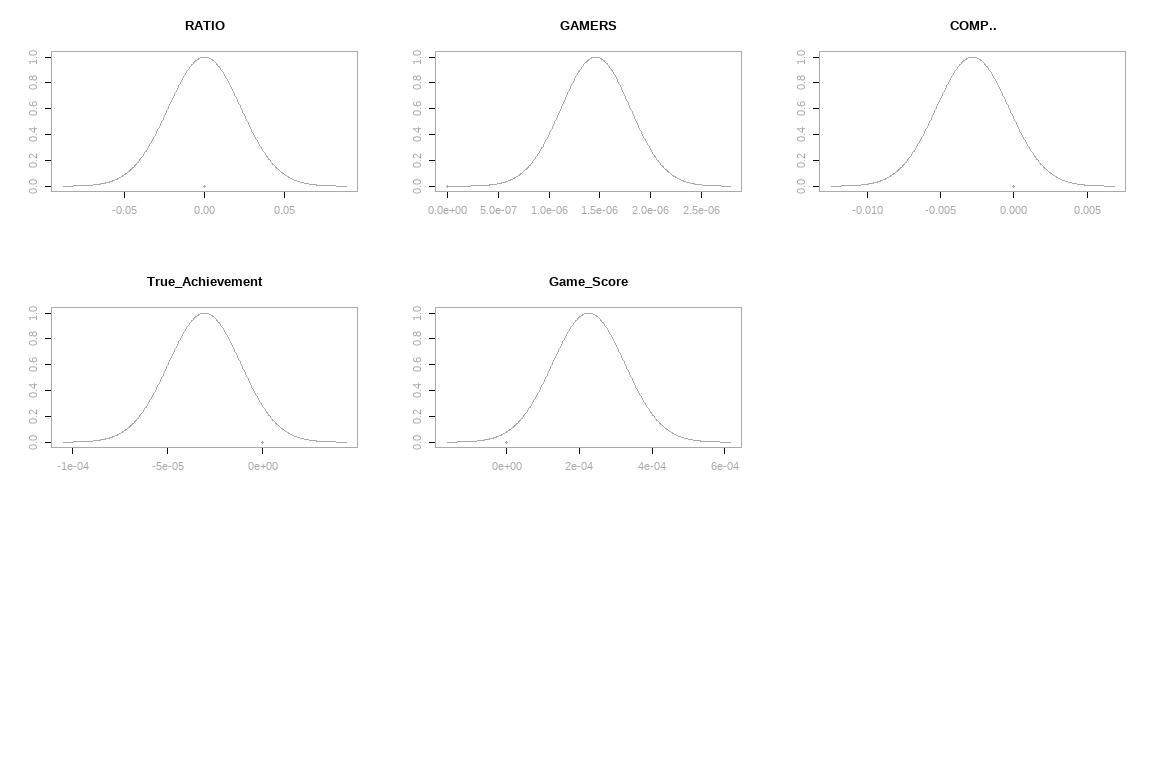
\includegraphics{Xbox_Games_Pass_files/figure-latex/unnamed-chunk-18-1.pdf}

\begin{Shaded}
\begin{Highlighting}[]
\CommentTok{#Credible interval}
\KeywordTok{confint}\NormalTok{(Games.coef,}\DataTypeTok{parm=}\DecValTok{2}\OperatorTok{:}\DecValTok{6}\NormalTok{)}
\end{Highlighting}
\end{Shaded}

\begin{verbatim}
##                           2.5%        97.5%          beta
## RATIO            -4.465320e-02 4.489955e-02  1.231774e-04
## GAMERS            7.924027e-07 2.127023e-06  1.459713e-06
## COMP..           -7.680424e-03 2.064663e-03 -2.807880e-03
## True_Achievement -6.829666e-05 7.018107e-06 -3.063928e-05
## Game_Score        2.901776e-05 4.219359e-04  2.254768e-04
## attr(,"Probability")
## [1] 0.95
## attr(,"class")
## [1] "confint.bas"
\end{verbatim}

\begin{Shaded}
\begin{Highlighting}[]
\CommentTok{##Since 0 is included within credible interval ratio,comp.. and true achievement are not significant to the model}


\NormalTok{out =}\StringTok{ }\KeywordTok{confint}\NormalTok{(Games.coef)[,}\DecValTok{1}\OperatorTok{:}\DecValTok{2}\NormalTok{]}
\CommentTok{# Extract the upper and lower bounds of the credible intervals}
\NormalTok{names =}\StringTok{ }\KeywordTok{c}\NormalTok{(}\StringTok{"posterior mean"}\NormalTok{, }\StringTok{"posterior std"}\NormalTok{, }\KeywordTok{colnames}\NormalTok{(out))}
\NormalTok{out =}\StringTok{ }\KeywordTok{cbind}\NormalTok{(Games.coef}\OperatorTok{$}\NormalTok{postmean, Games.coef}\OperatorTok{$}\NormalTok{postsd, out)}
\KeywordTok{colnames}\NormalTok{(out) =}\StringTok{ }\NormalTok{names}
\KeywordTok{round}\NormalTok{(out, }\DecValTok{2}\NormalTok{)}
\end{Highlighting}
\end{Shaded}

\begin{verbatim}
##                  posterior mean posterior std  2.5% 97.5%
## Intercept                  3.71          0.03  3.66  3.76
## RATIO                      0.00          0.02 -0.04  0.04
## GAMERS                     0.00          0.00  0.00  0.00
## COMP..                     0.00          0.00 -0.01  0.00
## True_Achievement           0.00          0.00  0.00  0.00
## Game_Score                 0.00          0.00  0.00  0.00
\end{verbatim}

\begin{Shaded}
\begin{Highlighting}[]
\CommentTok{#select the best model}
\CommentTok{#AIc}
\NormalTok{n=}\KeywordTok{nrow}\NormalTok{(training)}
\NormalTok{Games.lm=}\KeywordTok{lm}\NormalTok{(RATING }\OperatorTok{~}\NormalTok{.,}\DataTypeTok{data=}\NormalTok{training[}\OperatorTok{-}\KeywordTok{c}\NormalTok{(}\DecValTok{1}\NormalTok{,}\DecValTok{6}\NormalTok{)])}
\NormalTok{Games.step=}\KeywordTok{step}\NormalTok{(Games.lm,}\DataTypeTok{k=}\KeywordTok{log}\NormalTok{(n))}
\end{Highlighting}
\end{Shaded}

\begin{verbatim}
## Start:  AIC=-489.12
## RATING ~ RATIO + GAMERS + COMP.. + True_Achievement + Game_Score
## 
##                    Df Sum of Sq    RSS     AIC
## - RATIO             1    0.0000 71.706 -494.95
## - COMP..            1    0.2775 71.983 -493.64
## - True_Achievement  1    0.5533 72.259 -492.35
## - Game_Score        1    1.1009 72.807 -489.80
## <none>                          71.706 -489.12
## - GAMERS            1    3.9991 75.705 -476.60
## 
## Step:  AIC=-494.95
## RATING ~ GAMERS + COMP.. + True_Achievement + Game_Score
## 
##                    Df Sum of Sq    RSS     AIC
## - COMP..            1    0.2891 71.995 -499.41
## <none>                          71.706 -494.95
## - Game_Score        1    3.1389 74.845 -486.29
## - True_Achievement  1    3.8194 75.525 -483.23
## - GAMERS            1    4.0001 75.706 -482.42
## 
## Step:  AIC=-499.41
## RATING ~ GAMERS + True_Achievement + Game_Score
## 
##                    Df Sum of Sq    RSS     AIC
## <none>                          71.995 -499.41
## - Game_Score        1    2.9720 74.967 -491.56
## - True_Achievement  1    3.5321 75.527 -489.04
## - GAMERS            1    4.3084 76.303 -485.59
\end{verbatim}

\begin{Shaded}
\begin{Highlighting}[]
\NormalTok{Games.BIC=}\KeywordTok{bas.lm}\NormalTok{(RATING}\OperatorTok{~}\NormalTok{.,}\DataTypeTok{data=}\NormalTok{training[}\OperatorTok{-}\KeywordTok{c}\NormalTok{(}\DecValTok{1}\NormalTok{,}\DecValTok{6}\NormalTok{)],}\DataTypeTok{prior=}\StringTok{"BIC"}\NormalTok{,}\DataTypeTok{modelprior =} \KeywordTok{tr.beta.binomial}\NormalTok{(}\DecValTok{1}\NormalTok{,}\DecValTok{1}\NormalTok{,}\DecValTok{5}\NormalTok{))}
\NormalTok{Games.BIC}
\end{Highlighting}
\end{Shaded}

\begin{verbatim}
## 
## Call:
## bas.lm(formula = RATING ~ ., data = training[-c(1, 6)], prior = "BIC", 
##     modelprior = tr.beta.binomial(1, 1, 5))
## 
## 
##  Marginal Posterior Inclusion Probabilities: 
##        Intercept             RATIO            GAMERS            COMP..  
##           1.0000            0.4967            0.9995            0.1690  
## True_Achievement        Game_Score  
##           0.5605            0.6407
\end{verbatim}

\begin{Shaded}
\begin{Highlighting}[]
\NormalTok{best=}\KeywordTok{which.max}\NormalTok{(Games.BIC}\OperatorTok{$}\NormalTok{logmarg)}

\NormalTok{bestmodel=Games.BIC}\OperatorTok{$}\NormalTok{which[[best]]}
\NormalTok{bestmodel}
\end{Highlighting}
\end{Shaded}

\begin{verbatim}
## [1] 0 2 4 5
\end{verbatim}

\begin{Shaded}
\begin{Highlighting}[]
\NormalTok{bestgamma=}\KeywordTok{rep}\NormalTok{(}\DecValTok{0}\NormalTok{, Games.BIC}\OperatorTok{$}\NormalTok{n.vars)}
\NormalTok{bestgamma[bestmodel}\OperatorTok{+}\DecValTok{1}\NormalTok{]=}\DecValTok{1}
\NormalTok{bestgamma}
\end{Highlighting}
\end{Shaded}

\begin{verbatim}
## [1] 1 0 1 0 1 1
\end{verbatim}

\begin{Shaded}
\begin{Highlighting}[]
\CommentTok{#summary of best 5 models}
\NormalTok{Games_bas=}\KeywordTok{bas.lm}\NormalTok{(RATING}\OperatorTok{~}\NormalTok{GAMERS}\OperatorTok{+}\NormalTok{True_Achievement}\OperatorTok{+}\NormalTok{Game_Score,}\DataTypeTok{data=}\NormalTok{training[}\OperatorTok{-}\KeywordTok{c}\NormalTok{(}\DecValTok{1}\NormalTok{,}\DecValTok{6}\NormalTok{),],}\DataTypeTok{prior=}\StringTok{"BIC"}\NormalTok{,}\DataTypeTok{modelprior =} \KeywordTok{tr.beta.binomial}\NormalTok{(}\DecValTok{1}\NormalTok{,}\DecValTok{1}\NormalTok{,}\DecValTok{5}\NormalTok{))}
\KeywordTok{round}\NormalTok{(}\KeywordTok{summary}\NormalTok{(Games_bas),}\DecValTok{3}\NormalTok{)}
\end{Highlighting}
\end{Shaded}

\begin{verbatim}
##                  P(B != 0 | Y)  model 1  model 2  model 3  model 4 model 5
## Intercept                1.000    1.000    1.000    1.000    1.000    1.00
## GAMERS                   1.000    1.000    1.000    1.000    1.000    0.00
## True_Achievement         0.943    1.000    0.000    1.000    0.000    1.00
## Game_Score               0.924    1.000    0.000    0.000    1.000    1.00
## BF                          NA    1.000    0.171    0.077    0.016    0.00
## PostProbs                   NA    0.919    0.052    0.023    0.005    0.00
## R2                          NA    0.164    0.125    0.136    0.128    0.11
## dim                         NA    4.000    2.000    3.000    3.000    3.00
## logmarg                     NA -726.943 -728.707 -729.513 -731.109 -734.58
\end{verbatim}

\begin{Shaded}
\begin{Highlighting}[]
\CommentTok{##BIC is lower the better. logmarg=(-1/2BIC).logmarg higher the better}
\KeywordTok{print}\NormalTok{(Games_bas)}
\end{Highlighting}
\end{Shaded}

\begin{verbatim}
## 
## Call:
## bas.lm(formula = RATING ~ GAMERS + True_Achievement + Game_Score, 
##     data = training[-c(1, 6), ], prior = "BIC", modelprior = tr.beta.binomial(1, 
##         1, 5))
## 
## 
##  Marginal Posterior Inclusion Probabilities: 
##        Intercept            GAMERS  True_Achievement        Game_Score  
##           1.0000            0.9999            0.9428            0.9241
\end{verbatim}

\begin{Shaded}
\begin{Highlighting}[]
\CommentTok{#model validation}
\CommentTok{#Predict testing set}
\NormalTok{Predict <-}\StringTok{ }\KeywordTok{predict}\NormalTok{(Games_bas,}\DataTypeTok{newdata =}\NormalTok{ testing[}\OperatorTok{-}\KeywordTok{c}\NormalTok{(}\DecValTok{1}\NormalTok{,}\DecValTok{6}\NormalTok{)] )}
\CommentTok{#Compute errors}
\NormalTok{Error=testing}\OperatorTok{$}\NormalTok{RATING}\OperatorTok{-}\NormalTok{Predict}\OperatorTok{$}\NormalTok{fit}
\CommentTok{#Error}
\CommentTok{#RMSE}
\NormalTok{RMSE=}\KeywordTok{sqrt}\NormalTok{(}\KeywordTok{mean}\NormalTok{(Error}\OperatorTok{^}\DecValTok{2}\NormalTok{))}
\NormalTok{RMSE}
\end{Highlighting}
\end{Shaded}

\begin{verbatim}
## [1] 0.4662949
\end{verbatim}

\begin{Shaded}
\begin{Highlighting}[]
\NormalTok{Games.coef2=}\KeywordTok{coef}\NormalTok{(Games_bas)}
\KeywordTok{confint}\NormalTok{(Games.coef2)}
\end{Highlighting}
\end{Shaded}

\begin{verbatim}
##                           2.5%        97.5%          beta
## Intercept         3.654946e+00 3.753874e+00  3.701190e+00
## GAMERS            9.326980e-07 2.340336e-06  1.598260e-06
## True_Achievement -3.734677e-05 0.000000e+00 -2.440489e-05
## Game_Score        0.000000e+00 2.955501e-04  1.819028e-04
## attr(,"Probability")
## [1] 0.95
## attr(,"class")
## [1] "confint.bas"
\end{verbatim}

\begin{Shaded}
\begin{Highlighting}[]
\KeywordTok{par}\NormalTok{(}\DataTypeTok{mfrow =} \KeywordTok{c}\NormalTok{(}\DecValTok{2}\NormalTok{, }\DecValTok{2}\NormalTok{), }\DataTypeTok{col.lab =} \StringTok{"darkgrey"}\NormalTok{, }\DataTypeTok{col.axis =} \StringTok{"darkgrey"}\NormalTok{, }\DataTypeTok{col =} \StringTok{"darkgrey"}\NormalTok{)}
\KeywordTok{plot}\NormalTok{(Games.coef2, }\DataTypeTok{subset =} \DecValTok{2}\OperatorTok{:}\DecValTok{4}\NormalTok{, }\DataTypeTok{ask =}\NormalTok{ F)}
\end{Highlighting}
\end{Shaded}

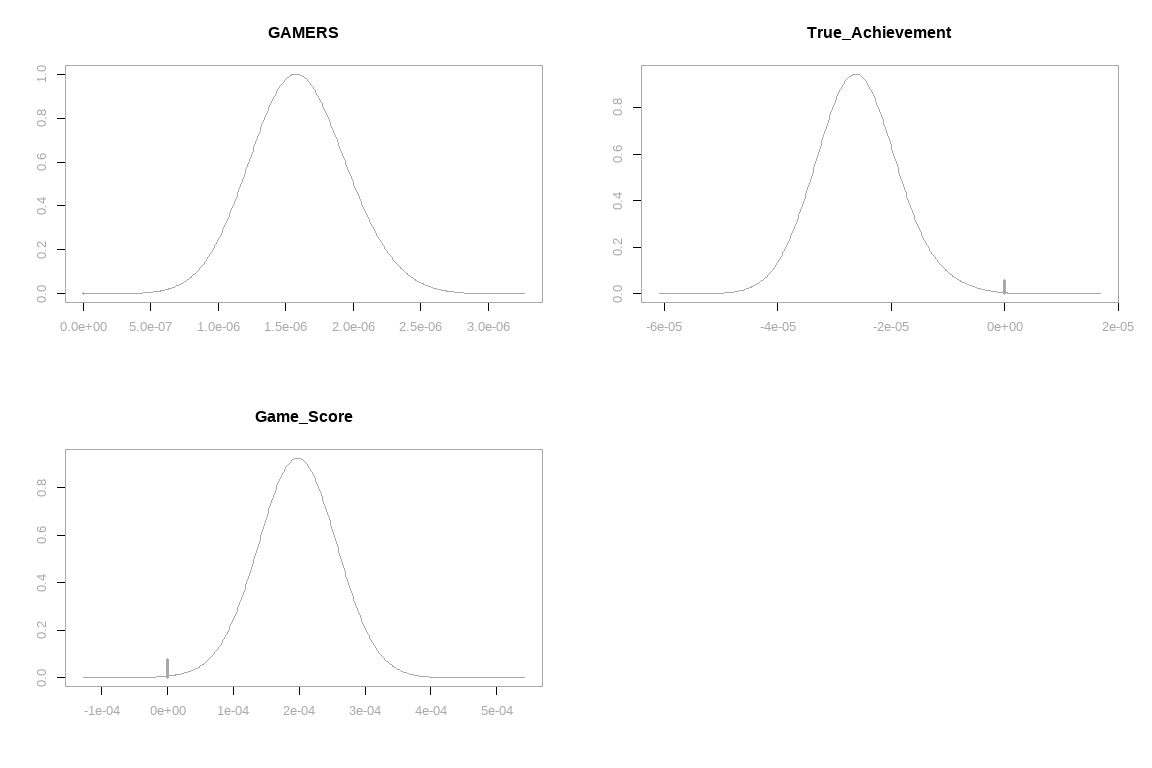
\includegraphics{Xbox_Games_Pass_files/figure-latex/unnamed-chunk-29-1.pdf}

\end{document}
